% Options for packages loaded elsewhere
\PassOptionsToPackage{unicode}{hyperref}
\PassOptionsToPackage{hyphens}{url}
\PassOptionsToPackage{dvipsnames,svgnames,x11names}{xcolor}
%
\documentclass[
  11pt,
]{article}

\usepackage{amsmath,amssymb}
\usepackage{iftex}
\ifPDFTeX
  \usepackage[T1]{fontenc}
  \usepackage[utf8]{inputenc}
  \usepackage{textcomp} % provide euro and other symbols
\else % if luatex or xetex
  \usepackage{unicode-math}
  \defaultfontfeatures{Scale=MatchLowercase}
  \defaultfontfeatures[\rmfamily]{Ligatures=TeX,Scale=1}
\fi
\usepackage{lmodern}
\ifPDFTeX\else  
    % xetex/luatex font selection
\fi
% Use upquote if available, for straight quotes in verbatim environments
\IfFileExists{upquote.sty}{\usepackage{upquote}}{}
\IfFileExists{microtype.sty}{% use microtype if available
  \usepackage[]{microtype}
  \UseMicrotypeSet[protrusion]{basicmath} % disable protrusion for tt fonts
}{}
\makeatletter
\@ifundefined{KOMAClassName}{% if non-KOMA class
  \IfFileExists{parskip.sty}{%
    \usepackage{parskip}
  }{% else
    \setlength{\parindent}{0pt}
    \setlength{\parskip}{6pt plus 2pt minus 1pt}}
}{% if KOMA class
  \KOMAoptions{parskip=half}}
\makeatother
\usepackage{xcolor}
\usepackage[margin=1in]{geometry}
\setlength{\emergencystretch}{3em} % prevent overfull lines
\setcounter{secnumdepth}{5}
% Make \paragraph and \subparagraph free-standing
\ifx\paragraph\undefined\else
  \let\oldparagraph\paragraph
  \renewcommand{\paragraph}[1]{\oldparagraph{#1}\mbox{}}
\fi
\ifx\subparagraph\undefined\else
  \let\oldsubparagraph\subparagraph
  \renewcommand{\subparagraph}[1]{\oldsubparagraph{#1}\mbox{}}
\fi

\usepackage{color}
\usepackage{fancyvrb}
\newcommand{\VerbBar}{|}
\newcommand{\VERB}{\Verb[commandchars=\\\{\}]}
\DefineVerbatimEnvironment{Highlighting}{Verbatim}{commandchars=\\\{\}}
% Add ',fontsize=\small' for more characters per line
\usepackage{framed}
\definecolor{shadecolor}{RGB}{241,243,245}
\newenvironment{Shaded}{\begin{snugshade}}{\end{snugshade}}
\newcommand{\AlertTok}[1]{\textcolor[rgb]{0.68,0.00,0.00}{#1}}
\newcommand{\AnnotationTok}[1]{\textcolor[rgb]{0.37,0.37,0.37}{#1}}
\newcommand{\AttributeTok}[1]{\textcolor[rgb]{0.40,0.45,0.13}{#1}}
\newcommand{\BaseNTok}[1]{\textcolor[rgb]{0.68,0.00,0.00}{#1}}
\newcommand{\BuiltInTok}[1]{\textcolor[rgb]{0.00,0.23,0.31}{#1}}
\newcommand{\CharTok}[1]{\textcolor[rgb]{0.13,0.47,0.30}{#1}}
\newcommand{\CommentTok}[1]{\textcolor[rgb]{0.37,0.37,0.37}{#1}}
\newcommand{\CommentVarTok}[1]{\textcolor[rgb]{0.37,0.37,0.37}{\textit{#1}}}
\newcommand{\ConstantTok}[1]{\textcolor[rgb]{0.56,0.35,0.01}{#1}}
\newcommand{\ControlFlowTok}[1]{\textcolor[rgb]{0.00,0.23,0.31}{#1}}
\newcommand{\DataTypeTok}[1]{\textcolor[rgb]{0.68,0.00,0.00}{#1}}
\newcommand{\DecValTok}[1]{\textcolor[rgb]{0.68,0.00,0.00}{#1}}
\newcommand{\DocumentationTok}[1]{\textcolor[rgb]{0.37,0.37,0.37}{\textit{#1}}}
\newcommand{\ErrorTok}[1]{\textcolor[rgb]{0.68,0.00,0.00}{#1}}
\newcommand{\ExtensionTok}[1]{\textcolor[rgb]{0.00,0.23,0.31}{#1}}
\newcommand{\FloatTok}[1]{\textcolor[rgb]{0.68,0.00,0.00}{#1}}
\newcommand{\FunctionTok}[1]{\textcolor[rgb]{0.28,0.35,0.67}{#1}}
\newcommand{\ImportTok}[1]{\textcolor[rgb]{0.00,0.46,0.62}{#1}}
\newcommand{\InformationTok}[1]{\textcolor[rgb]{0.37,0.37,0.37}{#1}}
\newcommand{\KeywordTok}[1]{\textcolor[rgb]{0.00,0.23,0.31}{#1}}
\newcommand{\NormalTok}[1]{\textcolor[rgb]{0.00,0.23,0.31}{#1}}
\newcommand{\OperatorTok}[1]{\textcolor[rgb]{0.37,0.37,0.37}{#1}}
\newcommand{\OtherTok}[1]{\textcolor[rgb]{0.00,0.23,0.31}{#1}}
\newcommand{\PreprocessorTok}[1]{\textcolor[rgb]{0.68,0.00,0.00}{#1}}
\newcommand{\RegionMarkerTok}[1]{\textcolor[rgb]{0.00,0.23,0.31}{#1}}
\newcommand{\SpecialCharTok}[1]{\textcolor[rgb]{0.37,0.37,0.37}{#1}}
\newcommand{\SpecialStringTok}[1]{\textcolor[rgb]{0.13,0.47,0.30}{#1}}
\newcommand{\StringTok}[1]{\textcolor[rgb]{0.13,0.47,0.30}{#1}}
\newcommand{\VariableTok}[1]{\textcolor[rgb]{0.07,0.07,0.07}{#1}}
\newcommand{\VerbatimStringTok}[1]{\textcolor[rgb]{0.13,0.47,0.30}{#1}}
\newcommand{\WarningTok}[1]{\textcolor[rgb]{0.37,0.37,0.37}{\textit{#1}}}

\providecommand{\tightlist}{%
  \setlength{\itemsep}{0pt}\setlength{\parskip}{0pt}}\usepackage{longtable,booktabs,array}
\usepackage{calc} % for calculating minipage widths
% Correct order of tables after \paragraph or \subparagraph
\usepackage{etoolbox}
\makeatletter
\patchcmd\longtable{\par}{\if@noskipsec\mbox{}\fi\par}{}{}
\makeatother
% Allow footnotes in longtable head/foot
\IfFileExists{footnotehyper.sty}{\usepackage{footnotehyper}}{\usepackage{footnote}}
\makesavenoteenv{longtable}
\usepackage{graphicx}
\makeatletter
\def\maxwidth{\ifdim\Gin@nat@width>\linewidth\linewidth\else\Gin@nat@width\fi}
\def\maxheight{\ifdim\Gin@nat@height>\textheight\textheight\else\Gin@nat@height\fi}
\makeatother
% Scale images if necessary, so that they will not overflow the page
% margins by default, and it is still possible to overwrite the defaults
% using explicit options in \includegraphics[width, height, ...]{}
\setkeys{Gin}{width=\maxwidth,height=\maxheight,keepaspectratio}
% Set default figure placement to htbp
\makeatletter
\def\fps@figure{htbp}
\makeatother

\makeatletter
\makeatother
\makeatletter
\makeatother
\makeatletter
\@ifpackageloaded{caption}{}{\usepackage{caption}}
\AtBeginDocument{%
\ifdefined\contentsname
  \renewcommand*\contentsname{Table of contents}
\else
  \newcommand\contentsname{Table of contents}
\fi
\ifdefined\listfigurename
  \renewcommand*\listfigurename{List of Figures}
\else
  \newcommand\listfigurename{List of Figures}
\fi
\ifdefined\listtablename
  \renewcommand*\listtablename{List of Tables}
\else
  \newcommand\listtablename{List of Tables}
\fi
\ifdefined\figurename
  \renewcommand*\figurename{Figure}
\else
  \newcommand\figurename{Figure}
\fi
\ifdefined\tablename
  \renewcommand*\tablename{Table}
\else
  \newcommand\tablename{Table}
\fi
}
\@ifpackageloaded{float}{}{\usepackage{float}}
\floatstyle{ruled}
\@ifundefined{c@chapter}{\newfloat{codelisting}{h}{lop}}{\newfloat{codelisting}{h}{lop}[chapter]}
\floatname{codelisting}{Listing}
\newcommand*\listoflistings{\listof{codelisting}{List of Listings}}
\makeatother
\makeatletter
\@ifpackageloaded{caption}{}{\usepackage{caption}}
\@ifpackageloaded{subcaption}{}{\usepackage{subcaption}}
\makeatother
\makeatletter
\@ifpackageloaded{tcolorbox}{}{\usepackage[skins,breakable]{tcolorbox}}
\makeatother
\makeatletter
\@ifundefined{shadecolor}{\definecolor{shadecolor}{rgb}{.97, .97, .97}}
\makeatother
\makeatletter
\makeatother
\makeatletter
\makeatother
\ifLuaTeX
  \usepackage{selnolig}  % disable illegal ligatures
\fi
\IfFileExists{bookmark.sty}{\usepackage{bookmark}}{\usepackage{hyperref}}
\IfFileExists{xurl.sty}{\usepackage{xurl}}{} % add URL line breaks if available
\urlstyle{same} % disable monospaced font for URLs
\hypersetup{
  pdftitle={Video Quality Analysis Report},
  colorlinks=true,
  linkcolor={blue},
  filecolor={Maroon},
  citecolor={Blue},
  urlcolor={Blue},
  pdfcreator={LaTeX via pandoc}}

\title{Video Quality Analysis Report}
\usepackage{etoolbox}
\makeatletter
\providecommand{\subtitle}[1]{% add subtitle to \maketitle
  \apptocmd{\@title}{\par {\large #1 \par}}{}{}
}
\makeatother
\subtitle{Flaco Owl Documentary Footage - Fifth Avenue Studios}
\author{}
\date{2025-11-13}

\begin{document}
\maketitle
\ifdefined\Shaded\renewenvironment{Shaded}{\begin{tcolorbox}[sharp corners, breakable, boxrule=0pt, frame hidden, borderline west={3pt}{0pt}{shadecolor}, interior hidden, enhanced]}{\end{tcolorbox}}\fi

\hypertarget{executive-summary}{%
\section{Executive Summary}\label{executive-summary}}

This report provides a comprehensive technical and narrative analysis of
video footage documenting Flaco the owl's first-night landing on Fifth
Avenue after being freed from the Central Park Zoo. The footage has been
evaluated for documentary production suitability, content significance,
and licensing valuation.

\textbf{Key Findings:}

\begin{longtable}[]{@{}ll@{}}
\toprule\noalign{}
Finding & Value \\
\midrule\noalign{}
\endhead
\bottomrule\noalign{}
\endlastfoot
Total Duration & 15.83 seconds \\
Usable Footage & 15.83 seconds (100\%) \\
High Quality Segments & 6.93 seconds (43.8\%) \\
Narrative Significance & 100/100 (CRITICAL) \\
Estimated Value Range & \$2,226 - \$2,713 \\
\end{longtable}

\hypertarget{technical-specifications}{%
\section{Technical Specifications}\label{technical-specifications}}

\begin{longtable}[]{@{}ll@{}}
\toprule\noalign{}
Property & Value \\
\midrule\noalign{}
\endhead
\bottomrule\noalign{}
\endlastfoot
Resolution & 720 × 1280 pixels (Full HD 1080p) \\
Frame Rate & 30.00 fps \\
Duration & 15.83 seconds \\
Total Frames & 475 frames \\
File Size & 4.76 MB \\
Codec & Unknown \\
Color Depth & 8-bit \\
\end{longtable}

\hypertarget{visual-quality-metrics}{%
\section{Visual Quality Metrics}\label{visual-quality-metrics}}

\begin{Shaded}
\begin{Highlighting}[]
\NormalTok{knitr}\SpecialCharTok{::}\FunctionTok{include\_graphics}\NormalTok{(}\StringTok{"figures/quality\_metrics\_radar.pdf"}\NormalTok{)}
\end{Highlighting}
\end{Shaded}

\begin{figure}[H]

{\centering 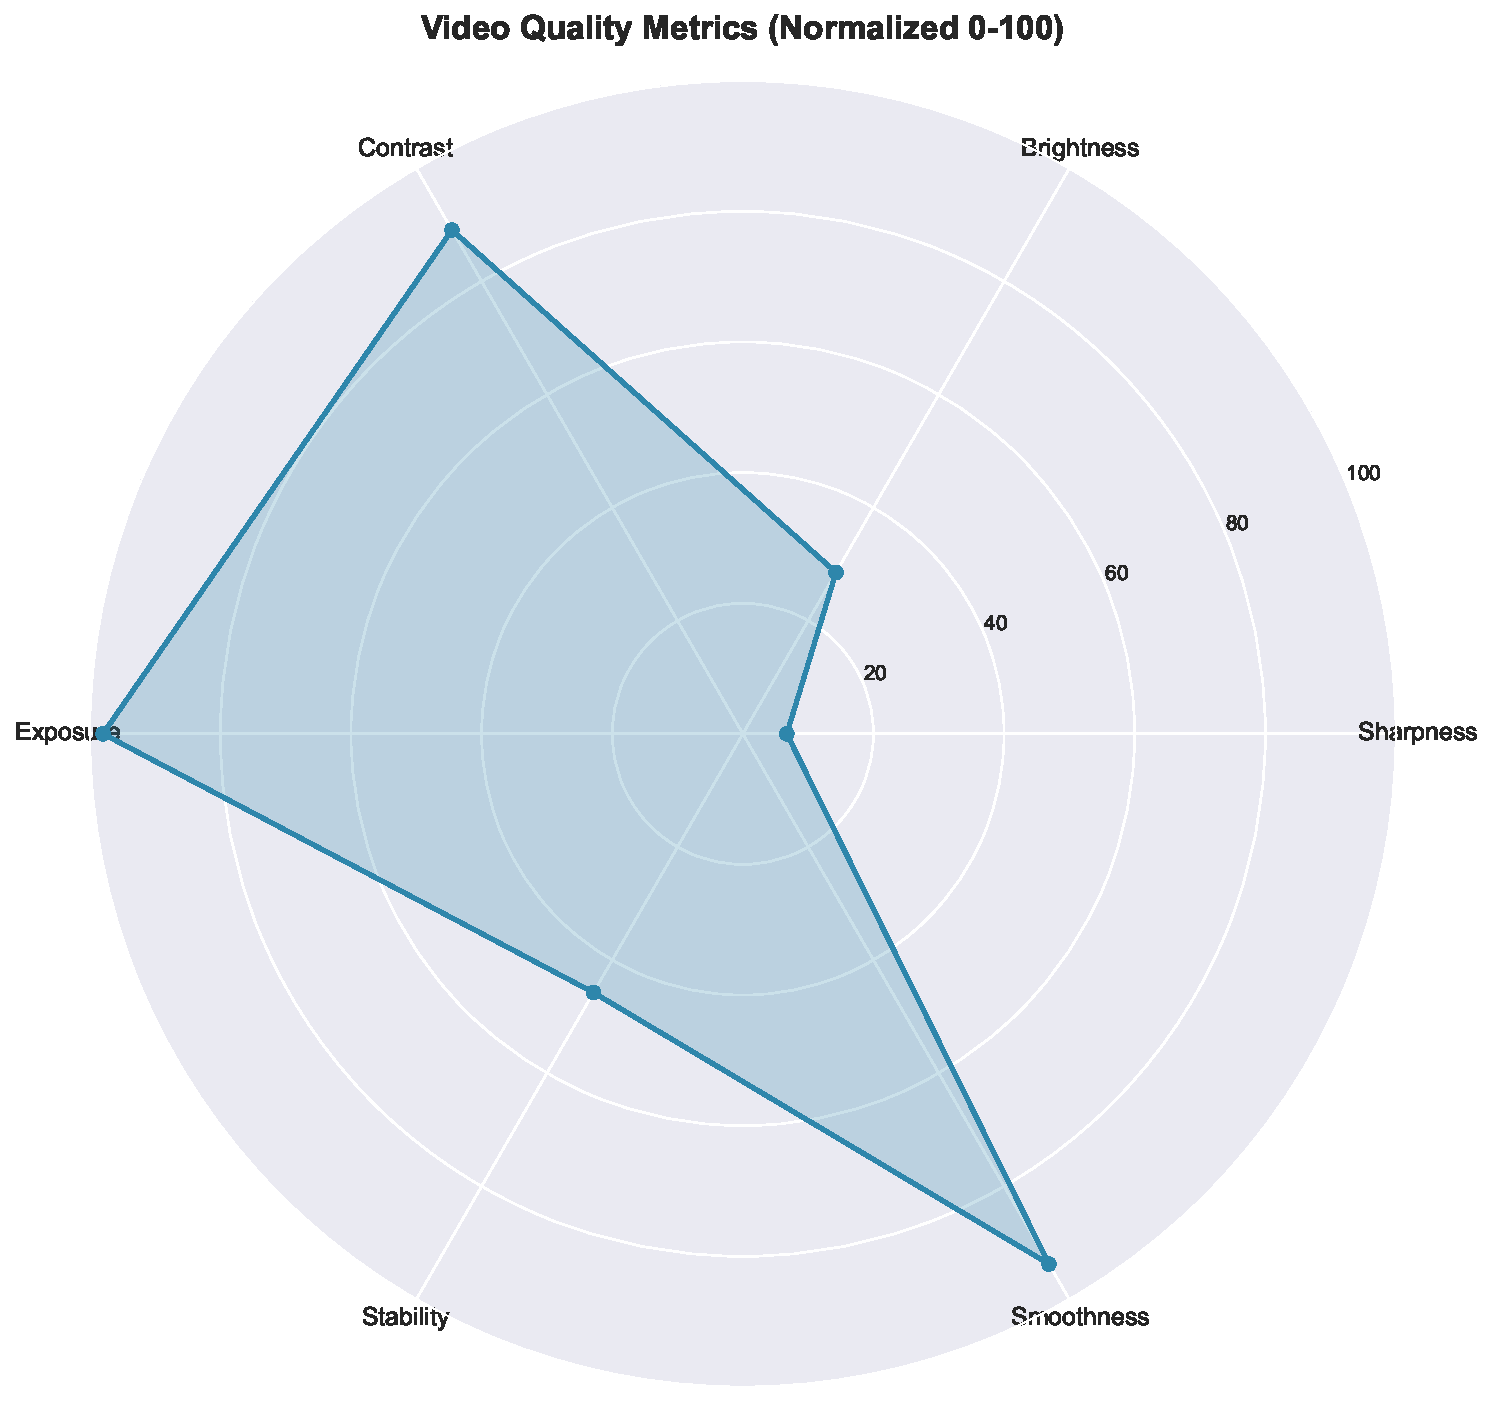
\includegraphics{figures/quality_metrics_radar.pdf}

}

\caption{\label{fig-quality-radar}Video Quality Metrics Radar Chart -
Normalized scores showing overall quality across key dimensions}

\end{figure}

\hypertarget{core-quality-metrics}{%
\subsection{Core Quality Metrics}\label{core-quality-metrics}}

\begin{longtable}[]{@{}lll@{}}
\toprule\noalign{}
Metric & Score & Assessment \\
\midrule\noalign{}
\endhead
\bottomrule\noalign{}
\endlastfoot
Sharpness & 33.65 & Very Soft/Blurry \\
Brightness & 72.8/255 & Underexposed \\
Contrast & 44.53 & High Contrast \\
Noise Level & 5.32 & Very Clean \\
Exposure & 98.0/100 & Excellent Exposure \\
Stability & 5.43 & Unstable/Shaky \\
Smoothness & 0.937 & Very Smooth \\
Color Compression & 0.876 & Minimal Compression \\
\end{longtable}

\hypertarget{quality-assessment}{%
\subsection{Quality Assessment}\label{quality-assessment}}

\textbf{Strengths:}

\begin{longtable}[]{@{}ll@{}}
\toprule\noalign{}
Strength & Description \\
\midrule\noalign{}
\endhead
\bottomrule\noalign{}
\endlastfoot
Resolution & High resolution (Full HD 1080p) suitable for broadcast \\
Exposure & Well-exposed footage with minimal over/under exposure \\
Noise Level & Clean footage with minimal noise (5.32) \\
Smoothness & Excellent temporal smoothness (0.937) \\
Compression & Minimal color compression artifacts (0.876) \\
\end{longtable}

\textbf{Issues Requiring Post-Processing:}

\begin{longtable}[]{@{}
  >{\raggedright\arraybackslash}p{(\columnwidth - 4\tabcolsep) * \real{0.1892}}
  >{\raggedright\arraybackslash}p{(\columnwidth - 4\tabcolsep) * \real{0.3514}}
  >{\raggedright\arraybackslash}p{(\columnwidth - 4\tabcolsep) * \real{0.4595}}@{}}
\toprule\noalign{}
\begin{minipage}[b]{\linewidth}\raggedright
Issue
\end{minipage} & \begin{minipage}[b]{\linewidth}\raggedright
Description
\end{minipage} & \begin{minipage}[b]{\linewidth}\raggedright
Required Action
\end{minipage} \\
\midrule\noalign{}
\endhead
\bottomrule\noalign{}
\endlastfoot
Sharpness & Footage is soft/blurry (sharpness: 33.65) & Requires
sharpening \\
Stability & Camera shake present (stability: 5.43) & Requires
stabilization \\
Brightness & Slightly underexposed (brightness: 72.8/255) & May need
color correction \\
\end{longtable}

\hypertarget{content-significance-analysis}{%
\section{Content Significance
Analysis}\label{content-significance-analysis}}

\hypertarget{subject-detection}{%
\subsection{Subject Detection}\label{subject-detection}}

\begin{Shaded}
\begin{Highlighting}[]
\NormalTok{knitr}\SpecialCharTok{::}\FunctionTok{include\_graphics}\NormalTok{(}\StringTok{"figures/content\_timeline.pdf"}\NormalTok{)}
\end{Highlighting}
\end{Shaded}

\begin{figure}[H]

{\centering 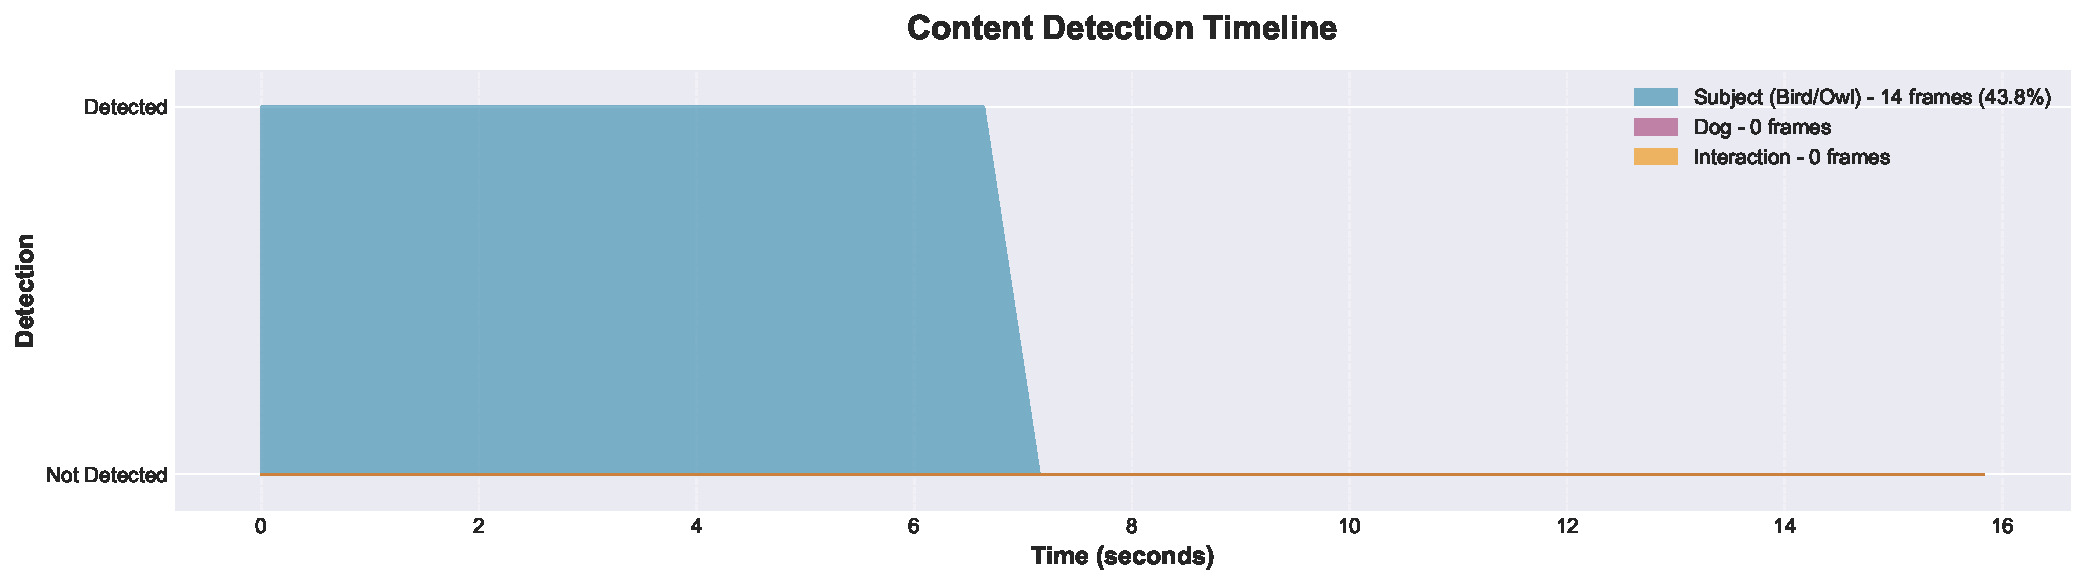
\includegraphics{figures/content_timeline.pdf}

}

\caption{\label{fig-content-timeline}Content Detection Timeline - When
the subject (bird/owl) appears throughout the video duration}

\end{figure}

\begin{longtable}[]{@{}ll@{}}
\toprule\noalign{}
Metric & Value \\
\midrule\noalign{}
\endhead
\bottomrule\noalign{}
\endlastfoot
Frames Analyzed & 32 frames \\
Frames with Subject (Bird/Owl) & 14 frames (43.8\%) \\
Frames with Dog & 0 frames \\
Frames with Interaction & 0 frames \\
Subject Visible Throughout & No \\
Interaction Moments Detected & No \\
Rare/Unique Event & Yes \\
\end{longtable}

\hypertarget{event-significance}{%
\subsection{Event Significance}\label{event-significance}}

This footage documents a \textbf{rare and historic event}: Flaco the
owl's first landing on Fifth Avenue on the night he was freed from the
Central Park Zoo. This represents a critical moment in the narrative arc
of the documentary, capturing the first public appearance of Flaco after
his escape.

\hypertarget{narrative-significance-story-value}{%
\section{Narrative Significance (Story
Value)}\label{narrative-significance-story-value}}

\hypertarget{narrative-score-100100-critical}{%
\subsection{Narrative Score: 100/100
(CRITICAL)}\label{narrative-score-100100-critical}}

\begin{Shaded}
\begin{Highlighting}[]
\NormalTok{knitr}\SpecialCharTok{::}\FunctionTok{include\_graphics}\NormalTok{(}\StringTok{"figures/narrative\_significance.pdf"}\NormalTok{)}
\end{Highlighting}
\end{Shaded}

\begin{figure}[H]

{\centering 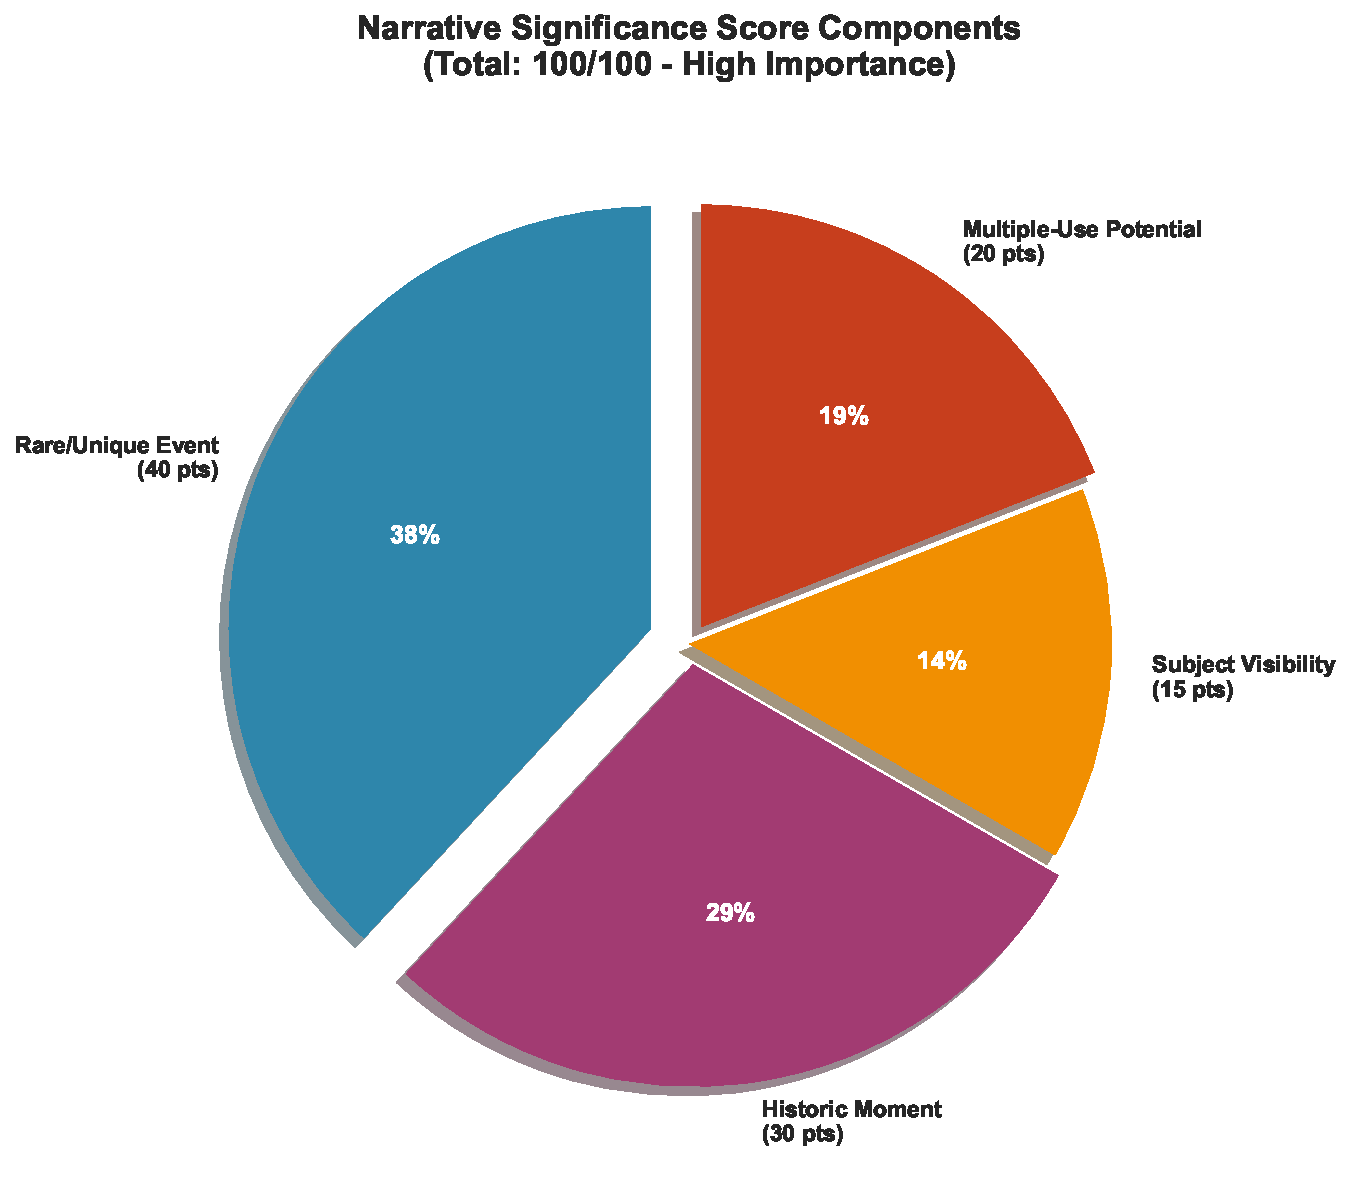
\includegraphics{figures/narrative_significance.pdf}

}

\caption{\label{fig-narrative}Narrative Significance Score Components -
Breakdown of factors contributing to the critical story importance
score}

\end{figure}

\begin{longtable}[]{@{}ll@{}}
\toprule\noalign{}
Factor & Contribution \\
\midrule\noalign{}
\endhead
\bottomrule\noalign{}
\endlastfoot
Rare/Unique Event & First-night landing on Fifth Ave \\
Historic Moment & First appearance after zoo escape \\
Subject Visibility & Subject visible in 44\% of footage \\
Multiple-Use Potential & Can be used multiple times in doc \\
Story Importance & CRITICAL \\
\end{longtable}

\textbf{Multiple-Use Potential:} This footage can be strategically
reused throughout the documentary in:

\begin{longtable}[]{@{}ll@{}}
\toprule\noalign{}
Use Case & Description \\
\midrule\noalign{}
\endhead
\bottomrule\noalign{}
\endlastfoot
Opening Sequence & Can be used in documentary opening \\
Transitional Moments & Suitable for scene transitions \\
Key Narrative Scenes & Can feature in critical story moments \\
Closing Sequences & Appropriate for documentary conclusion \\
\end{longtable}

\hypertarget{usability-analysis}{%
\section{Usability Analysis}\label{usability-analysis}}

\begin{Shaded}
\begin{Highlighting}[]
\NormalTok{knitr}\SpecialCharTok{::}\FunctionTok{include\_graphics}\NormalTok{(}\StringTok{"figures/usability\_breakdown.pdf"}\NormalTok{)}
\end{Highlighting}
\end{Shaded}

\begin{figure}[H]

{\centering 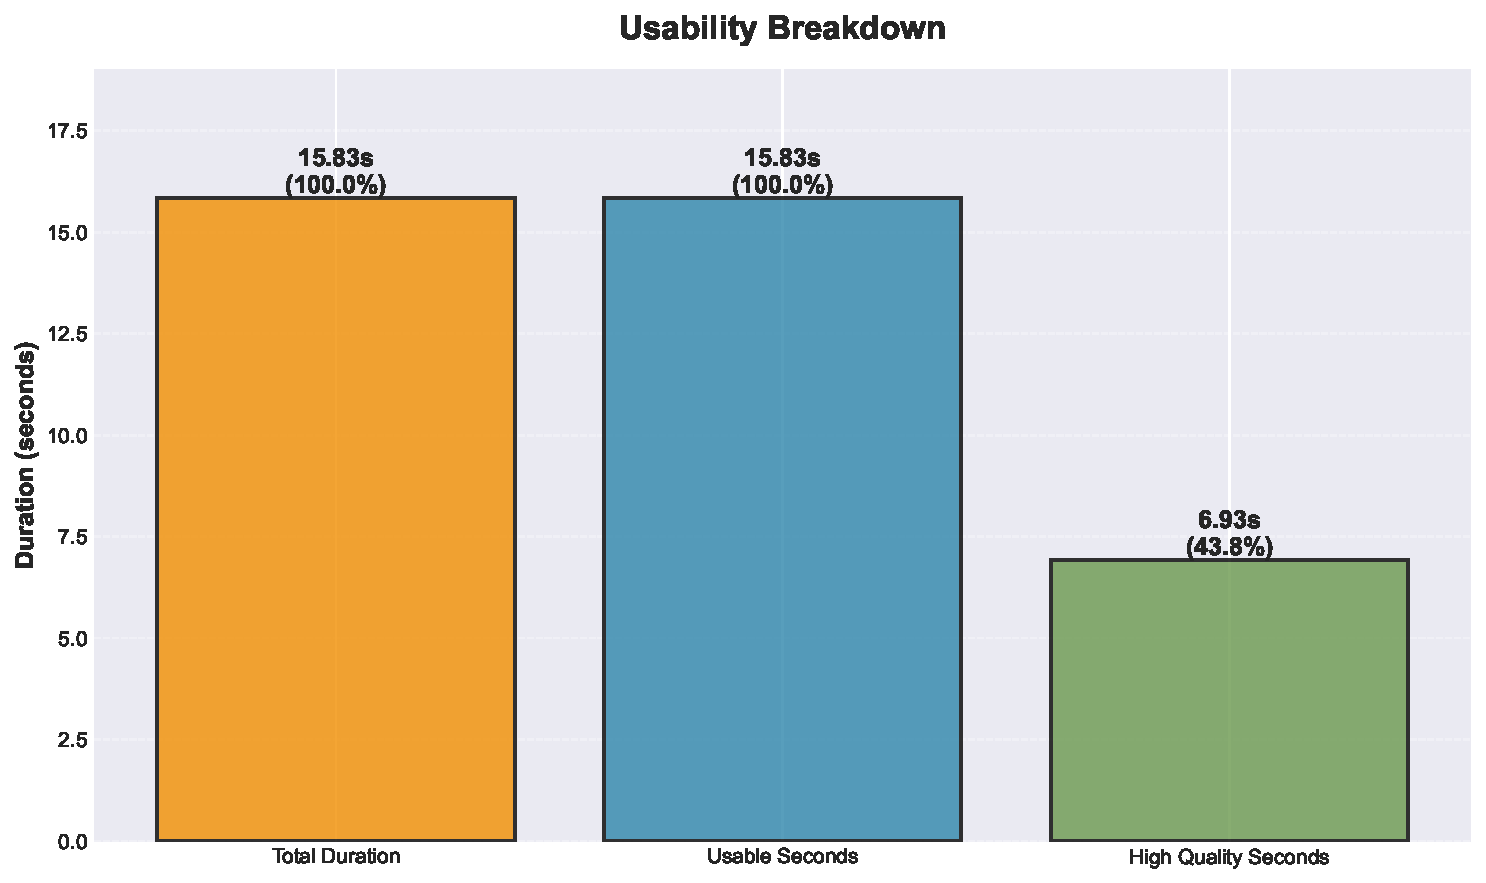
\includegraphics{figures/usability_breakdown.pdf}

}

\caption{\label{fig-usability}Usability Breakdown - Total duration,
usable seconds, and high-quality segments}

\end{figure}

\hypertarget{per-second-breakdown}{%
\subsection{Per-Second Breakdown}\label{per-second-breakdown}}

\begin{longtable}[]{@{}lll@{}}
\toprule\noalign{}
Category & Seconds & Percentage \\
\midrule\noalign{}
\endhead
\bottomrule\noalign{}
\endlastfoot
Total Duration & 15.83 & 100.0\% \\
Usable Seconds & 15.83 & 100.0\% \\
High Quality Seconds & 6.93 & 43.8\% \\
\end{longtable}

\textbf{Usable Segments:} 1 continuous segment (0.00s - 15.83s)

\hypertarget{clear-focused-segments}{%
\subsection{Clear, Focused Segments}\label{clear-focused-segments}}

No continuous clear/focused segments of 1 second or longer were
identified. The footage requires post-processing (sharpening and
stabilization) to achieve optimal clarity for broadcast use.

\hypertarget{valuation-guidance}{%
\section{Valuation Guidance}\label{valuation-guidance}}

\begin{Shaded}
\begin{Highlighting}[]
\NormalTok{knitr}\SpecialCharTok{::}\FunctionTok{include\_graphics}\NormalTok{(}\StringTok{"figures/valuation\_breakdown.pdf"}\NormalTok{)}
\end{Highlighting}
\end{Shaded}

\begin{figure}[H]

{\centering 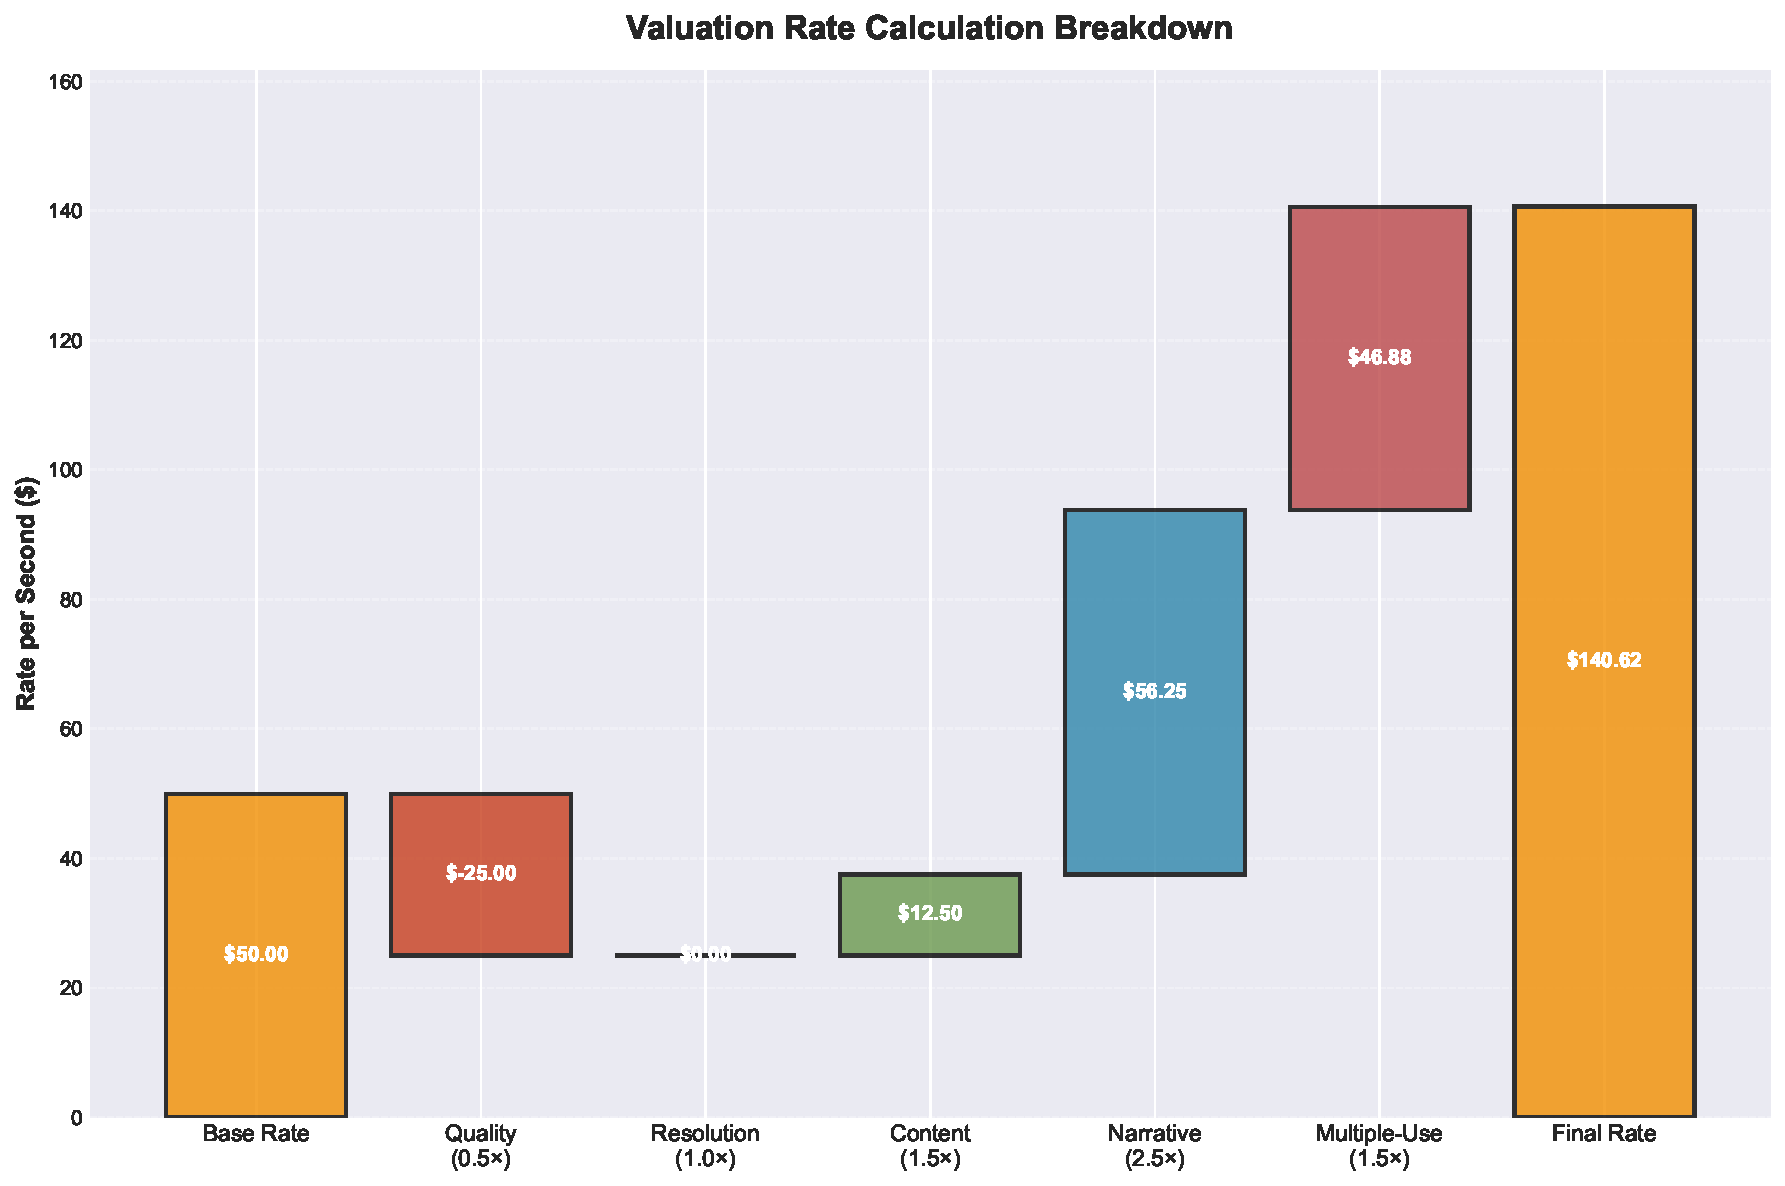
\includegraphics{figures/valuation_breakdown.pdf}

}

\caption{\label{fig-valuation-breakdown}Valuation Rate Calculation -
Step-by-step breakdown showing how multipliers affect the final rate per
second}

\end{figure}

\begin{Shaded}
\begin{Highlighting}[]
\NormalTok{knitr}\SpecialCharTok{::}\FunctionTok{include\_graphics}\NormalTok{(}\StringTok{"figures/value\_range.pdf"}\NormalTok{)}
\end{Highlighting}
\end{Shaded}

\begin{figure}[H]

{\centering 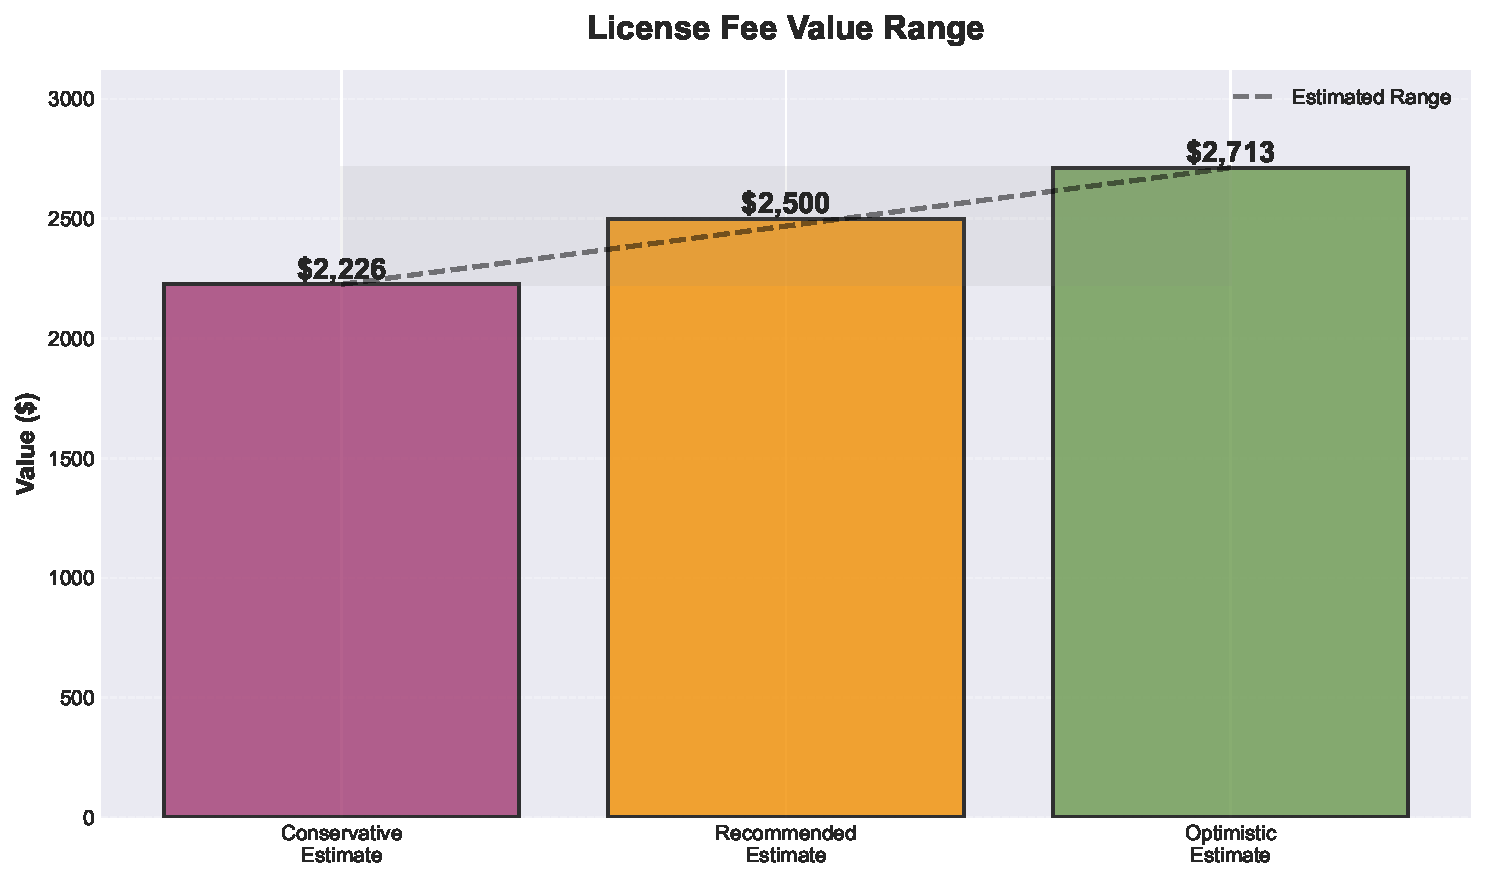
\includegraphics{figures/value_range.pdf}

}

\caption{\label{fig-value-range}License Fee Value Range - Conservative
estimate, agreed fee, and optimistic estimate comparison}

\end{figure}

\hypertarget{rate-calculation}{%
\subsection{Rate Calculation}\label{rate-calculation}}

\begin{longtable}[]{@{}lll@{}}
\toprule\noalign{}
Factor & Multiplier & Value \\
\midrule\noalign{}
\endhead
\bottomrule\noalign{}
\endlastfoot
Base Rate (per usable second) & 1.00× & \$50.00 \\
Quality Multiplier & 0.50× & \\
Resolution Multiplier & 1.00× & \\
Content Significance Multiplier & 1.50× & \\
Narrative Significance Multiplier & 2.50× & \\
Multiple-Use Multiplier & 1.50× & \\
\textbf{Final Rate per Second} & & \textbf{\$140.62} \\
\end{longtable}

\hypertarget{estimated-value-range}{%
\subsection{Estimated Value Range}\label{estimated-value-range}}

\begin{longtable}[]{@{}lll@{}}
\toprule\noalign{}
Estimate Type & Calculation & Value \\
\midrule\noalign{}
\endhead
\bottomrule\noalign{}
\endlastfoot
Conservative & All usable seconds × \$140.62 & \$2,226 \\
Optimistic & Premium segments at 1.5× rate & \$2,713 \\
\textbf{Recommended Range} & & \textbf{\$2,226 - \$2,713} \\
\end{longtable}

\hypertarget{valuation-notes}{%
\subsection{Valuation Notes}\label{valuation-notes}}

\begin{longtable}[]{@{}
  >{\raggedright\arraybackslash}p{(\columnwidth - 2\tabcolsep) * \real{0.3158}}
  >{\raggedright\arraybackslash}p{(\columnwidth - 2\tabcolsep) * \real{0.6842}}@{}}
\toprule\noalign{}
\begin{minipage}[b]{\linewidth}\raggedright
Note
\end{minipage} & \begin{minipage}[b]{\linewidth}\raggedright
Description
\end{minipage} \\
\midrule\noalign{}
\endhead
\bottomrule\noalign{}
\endlastfoot
Usability & High usability (100\% usable) - most of the clip is
production-ready \\
Archival Value & Rare/unique event adds significant archival and
narrative value \\
Post-Processing & Lower technical quality may require post-processing,
factor into negotiations \\
Story Value & Critical story moment with high reuse potential increases
value \\
Licensing Premium & Multiple-use licensing should command premium
rate \\
\end{longtable}

\hypertarget{recommendations}{%
\section{Recommendations}\label{recommendations}}

\hypertarget{for-licensing-negotiations}{%
\subsection{For Licensing
Negotiations}\label{for-licensing-negotiations}}

\begin{longtable}[]{@{}
  >{\raggedright\arraybackslash}p{(\columnwidth - 2\tabcolsep) * \real{0.5517}}
  >{\raggedright\arraybackslash}p{(\columnwidth - 2\tabcolsep) * \real{0.4483}}@{}}
\toprule\noalign{}
\begin{minipage}[b]{\linewidth}\raggedright
Recommendation
\end{minipage} & \begin{minipage}[b]{\linewidth}\raggedright
Description
\end{minipage} \\
\midrule\noalign{}
\endhead
\bottomrule\noalign{}
\endlastfoot
Base Value & Start with conservative estimate (\$2,226) as floor \\
Premium Value & Use optimistic estimate (\$2,713) for exclusive/premium
use \\
Multiple Uses & Factor in 1.5× multiplier for multiple-use licensing \\
Post-Processing & Consider that footage requires stabilization and
sharpening \\
Narrative Value & Emphasize critical story importance and archival
significance \\
\end{longtable}

\hypertarget{for-production-use}{%
\subsection{For Production Use}\label{for-production-use}}

\begin{longtable}[]{@{}
  >{\raggedright\arraybackslash}p{(\columnwidth - 2\tabcolsep) * \real{0.3333}}
  >{\raggedright\arraybackslash}p{(\columnwidth - 2\tabcolsep) * \real{0.6667}}@{}}
\toprule\noalign{}
\begin{minipage}[b]{\linewidth}\raggedright
Aspect
\end{minipage} & \begin{minipage}[b]{\linewidth}\raggedright
Recommendation
\end{minipage} \\
\midrule\noalign{}
\endhead
\bottomrule\noalign{}
\endlastfoot
Suitability & Footage is suitable for documentary use with
post-processing \\
Stabilization & Recommend stabilization software (e.g., Adobe Warp
Stabilizer) \\
Sharpening & Recommend sharpening filters to improve clarity \\
Color Correction & Color correction may enhance underexposed areas \\
Usage Flexibility & Footage can be used multiple times throughout
documentary structure \\
\end{longtable}

\hypertarget{conclusion}{%
\section{Conclusion}\label{conclusion}}

This footage represents a critical moment in Flaco the owl's story,
documenting his first landing on Fifth Avenue after being freed from the
Central Park Zoo. While the technical quality requires post-processing,
the narrative significance, rarity, and multiple-use potential make this
footage highly valuable for documentary production.

The estimated licensing value range of \$2,226 - \$2,713 reflects both
the technical quality considerations and the substantial narrative value
of this historic moment.

\newpage

\hypertarget{appendix-score-computation-methodology}{%
\section{Appendix: Score Computation
Methodology}\label{appendix-score-computation-methodology}}

\hypertarget{overall-quality-score}{%
\subsection{Overall Quality Score}\label{overall-quality-score}}

\begin{Shaded}
\begin{Highlighting}[]
\NormalTok{knitr}\SpecialCharTok{::}\FunctionTok{include\_graphics}\NormalTok{(}\StringTok{"figures/quality\_score\_components.pdf"}\NormalTok{)}
\end{Highlighting}
\end{Shaded}

\begin{figure}[H]

{\centering 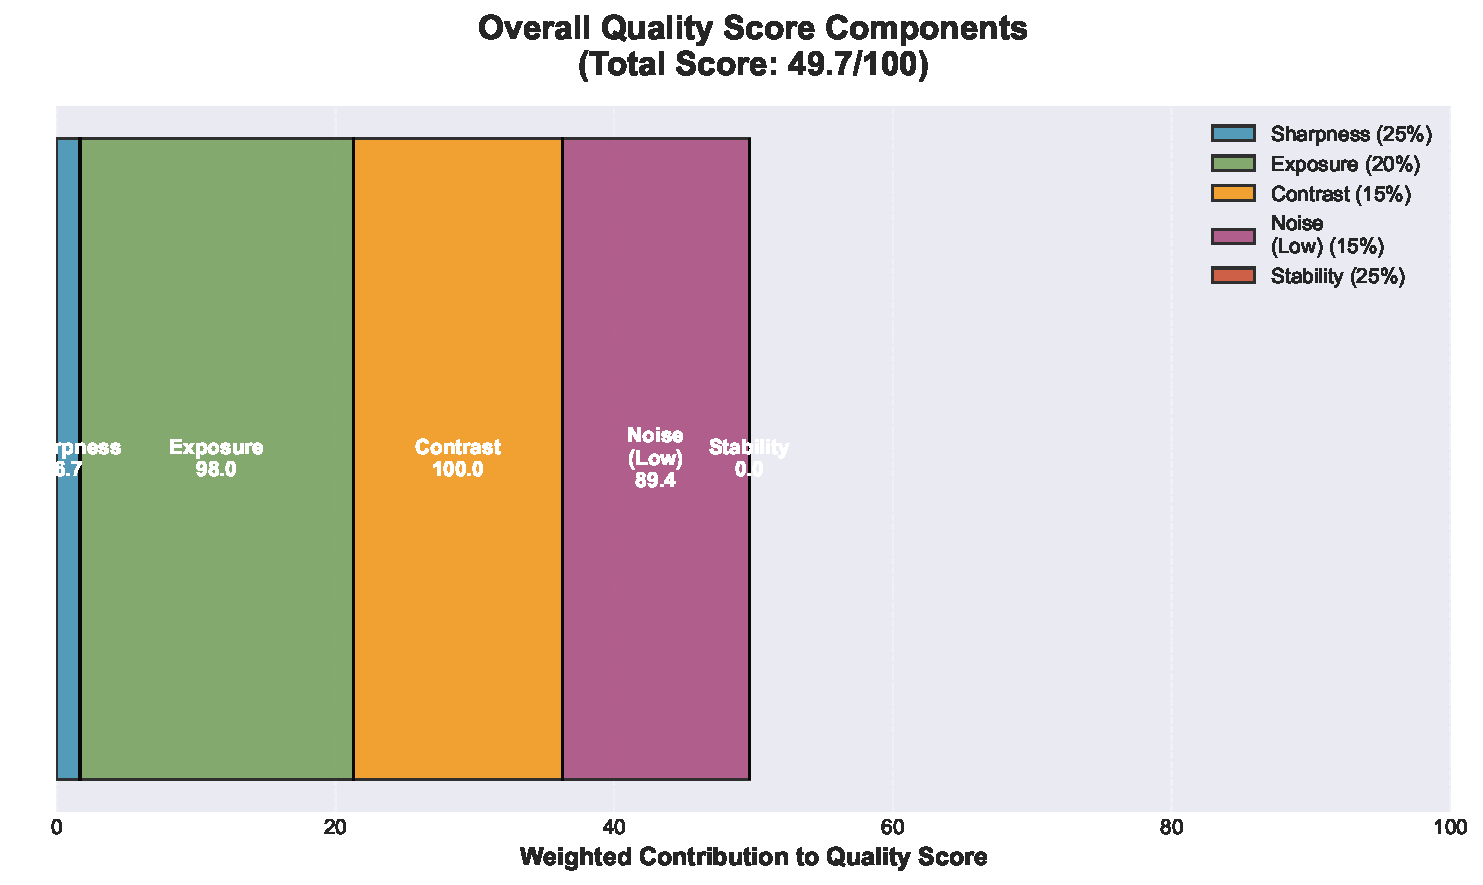
\includegraphics{figures/quality_score_components.pdf}

}

\caption{\label{fig-quality-components}Quality Score Components -
Weighted contribution of each metric to the overall quality score}

\end{figure}

The overall quality score is calculated using a weighted average of
normalized metrics:

\[Q = 0.25 \cdot S_n + 0.20 \cdot E_n + 0.15 \cdot C_n + 0.15 \cdot N_n + 0.25 \cdot St_n\]

Where:

\[S_n = \min\left(100, \frac{\bar{S}}{500} \times 100\right) \quad \text{(Sharpness, normalized)}\]

\[E_n = \bar{E} \quad \text{(Exposure score, 0-100)}\]

\[C_n = \min\left(100, \frac{\bar{C}}{40} \times 100\right) \quad \text{(Contrast, normalized)}\]

\[N_n = \max\left(0, 100 - \frac{\bar{N}}{50} \times 100\right) \quad \text{(Noise, normalized)}\]

\[St_n = \max\left(0, 100 - \frac{\bar{St}}{5} \times 100\right) \quad \text{(Stability, normalized)}\]

\hypertarget{sharpness-calculation}{%
\subsection{Sharpness Calculation}\label{sharpness-calculation}}

Sharpness is measured using Laplacian variance:

\[S = \text{Var}(\nabla^2 I)\]

Where \(\nabla^2 I\) is the Laplacian of the grayscale image \(I\).

\hypertarget{brightness-assessment}{%
\subsection{Brightness Assessment}\label{brightness-assessment}}

Average brightness is calculated as:

\[B = \frac{1}{N} \sum_{i,j} I_{gray}(i,j)\]

Assessment thresholds:

\begin{longtable}[]{@{}ll@{}}
\toprule\noalign{}
Category & Threshold \\
\midrule\noalign{}
\endhead
\bottomrule\noalign{}
\endlastfoot
Well-exposed & \(100 \leq B \leq 180\) \\
Underexposed & \(50 \leq B < 100\) \\
Very dark & \(B < 50\) \\
Overexposed & \(B > 200\) \\
\end{longtable}

\hypertarget{contrast-calculation}{%
\subsection{Contrast Calculation}\label{contrast-calculation}}

RMS contrast is calculated as:

\[C = \sqrt{\frac{1}{N} \sum_{i,j} (I_{gray}(i,j) - \mu)^2}\]

Where \(\mu\) is the mean brightness.

\hypertarget{noise-level-estimation}{%
\subsection{Noise Level Estimation}\label{noise-level-estimation}}

Noise level is estimated using the standard deviation of the Laplacian:

\[N = \sigma(\nabla^2 I)\]

\hypertarget{stability-calculation}{%
\subsection{Stability Calculation}\label{stability-calculation}}

Stability is measured using optical flow magnitude:

\[St = \frac{1}{M} \sum_{i,j} \sqrt{u(i,j)^2 + v(i,j)^2}\]

Where \((u, v)\) are the optical flow vectors between consecutive
frames.

\hypertarget{smoothness-calculation}{%
\subsection{Smoothness Calculation}\label{smoothness-calculation}}

Smoothness combines histogram similarity and color consistency:

\[Sm = \frac{H_{corr} + C_{cons}}{2}\]

Where:

\[H_{corr} = \text{Histogram correlation between frames}\]

\[C_{cons} = 1 - \frac{\bar{\Delta H}}{180} \quad \text{(Color consistency)}\]

\hypertarget{color-compression-score}{%
\subsection{Color Compression Score}\label{color-compression-score}}

Compression score is calculated as:

\[CC = 1 - \frac{B_h + B_s + B_v}{3}\]

Where \(B_h\), \(B_s\), \(B_v\) are banding scores for hue, saturation,
and value channels respectively.

\hypertarget{narrative-significance-score}{%
\subsection{Narrative Significance
Score}\label{narrative-significance-score}}

Narrative score is calculated as:

\[NS = \min(100, \sum_{i} w_i \cdot f_i)\]

Where \(w_i\) are weights and \(f_i\) are factors:

\begin{longtable}[]{@{}ll@{}}
\toprule\noalign{}
Factor & Points \\
\midrule\noalign{}
\endhead
\bottomrule\noalign{}
\endlastfoot
Rare/unique event & +40 points \\
Historic moment & +30 points \\
Subject visibility (\textgreater30\%) & +15 points \\
Clear focused segments (≥3s) & +10 points \\
Multiple clear segments & +5 points \\
Interaction moments & +10 points \\
Multiple-use potential & +20 points \\
\end{longtable}

\hypertarget{valuation-rate-calculation}{%
\subsection{Valuation Rate
Calculation}\label{valuation-rate-calculation}}

The final rate per usable second is calculated as:

\[R = R_{base} \times M_q \times M_r \times M_c \times M_n \times M_m\]

Where:

\[R_{base} = \$50 \quad \text{(Base rate)}\]

\[M_q = \text{Quality multiplier (0.5-2.0)}\]

\[M_r = \text{Resolution multiplier (0.5-1.5)}\]

\[M_c = \text{Content significance multiplier (1.0-1.8)}\]

\[M_n = \text{Narrative significance multiplier (1.0-2.5)}\]

\[M_m = \text{Multiple-use multiplier (1.0-1.5)}\]

\hypertarget{total-value-calculation}{%
\subsection{Total Value Calculation}\label{total-value-calculation}}

\[V_{conservative} = R \times T_{usable}\]

\[V_{optimistic} = R \times 1.5 \times T_{high} + R \times (T_{usable} - T_{high})\]

Where:

\begin{longtable}[]{@{}ll@{}}
\toprule\noalign{}
Variable & Description \\
\midrule\noalign{}
\endhead
\bottomrule\noalign{}
\endlastfoot
\(T_{usable}\) & Total usable seconds \\
\(T_{high}\) & High quality seconds \\
\end{longtable}

\hypertarget{technical-details}{%
\subsection{Technical Details}\label{technical-details}}

\hypertarget{analysis-parameters}{%
\subsubsection{Analysis Parameters}\label{analysis-parameters}}

\begin{longtable}[]{@{}ll@{}}
\toprule\noalign{}
Parameter & Value \\
\midrule\noalign{}
\endhead
\bottomrule\noalign{}
\endlastfoot
Frames sampled & 32 frames (2 frames per second) \\
Analysis method & Frame-by-frame quality assessment \\
Object detection & YOLOv8n model \\
Minimum segment duration & 1.0 second \\
Usability threshold & 35/100 points \\
High quality threshold & 60/100 points \\
\end{longtable}

\hypertarget{software-and-tools}{%
\subsubsection{Software and Tools}\label{software-and-tools}}

\begin{longtable}[]{@{}ll@{}}
\toprule\noalign{}
Tool & Purpose \\
\midrule\noalign{}
\endhead
\bottomrule\noalign{}
\endlastfoot
OpenCV 4.12.0 & Video processing \\
Ultralytics YOLOv8 & Object detection \\
NumPy & Numerical computations \\
Custom algorithms & Quality metrics analysis \\
\end{longtable}



\end{document}
